% This is sigproc-sp.tex -FILE FOR V2.6SP OF ACM_PROC_ARTICLE-SP.CLS
% OCTOBER 2002
%
% It is an example file showing how to use the 'acm_proc_article-sp.cls' V2.6SP
% LaTeX2e document class file for Conference Proceedings submissions.
% ----------------------------------------------------------------------------------------------------------------
% This .tex file (and associated .cls V2.6SP) *DOES NOT* produce:
%       1) The Permission Statement
%       2) The Conference (location) Info information
%       3) The Copyright Line with ACM data
%       4) Page numbering
%
%  However, both the CopyrightYear (default to 2002) and the ACM Copyright Data
% (default to X-XXXXX-XX-X/XX/XX) can still be over-ridden by whatever the author
% inserts into the source .tex file.
% e.g.
% \CopyrightYear{2003} will cause 2003 to appear in the copyright line.
% \crdata{0-12345-67-8/90/12} will cause 0-12345-67-8/90/12 to appear in the copyright line.
%
% ---------------------------------------------------------------------------------------------------------------
% It is an example which *does* use the .bib file (from which the .bbl file
% is produced).
% REMEMBER HOWEVER: After having produced the .bbl file,
% and prior to final submission,
% you need to 'insert'  your .bbl file into your source .tex file so as to provide
% ONE 'self-contained' source file.
%
% Questions regarding SIGS should be sent to
% Adrienne Griscti ---> griscti@acm.org
%
% Questions/suggestions regarding the guidelines, .tex and .cls files, etc. to
% Gerald Murray ---> murray@acm.org
%
% For tracking purposes - this is V2.6SP - OCTOBER 2002


% This is sigproc-sp.tex -FILE FOR V2.6SP OF ACM_PROC_ARTICLE-SP.CLS
% OCTOBER 2002
%
% It is an example file showing how to use the 'acm_proc_article-sp.cls' V2.6SP
% LaTeX2e document class file for Conference Proceedings submissions.
% ----------------------------------------------------------------------------------------------------------------
% This .tex file (and associated .cls V2.6SP) *DOES NOT* produce:
%       1) The Permission Statement
%       2) The Conference (location) Info information
%       3) The Copyright Line with ACM data
%       4) Page numbering
%
%  However, both the CopyrightYear (default to 2002) and the ACM Copyright Data
% (default to X-XXXXX-XX-X/XX/XX) can still be over-ridden by whatever the author
% inserts into the source .tex file.
% e.g.
% \CopyrightYear{2003} will cause 2003 to appear in the copyright line.
% \crdata{0-12345-67-8/90/12} will cause 0-12345-67-8/90/12 to appear in the copyright line.
%
% ---------------------------------------------------------------------------------------------------------------
% It is an example which *does* use the .bib file (from which the .bbl file
% is produced).
% REMEMBER HOWEVER: After having produced the .bbl file,
% and prior to final submission,
% you need to 'insert'  your .bbl file into your source .tex file so as to provide
% ONE 'self-contained' source file.
%
% Questions regarding SIGS should be sent to
% Adrienne Griscti ---> griscti@acm.org
%
% Questions/suggestions regarding the guidelines, .tex and .cls files, etc. to
% Gerald Murray ---> murray@acm.org
%
% For tracking purposes - this is V2.6SP - OCTOBER 2002


\documentclass{sig-alternate}

\usepackage{hyperref}
\usepackage{verbatim}


\begin{document}




%
% --- Author Metadata here ---
%\conferenceinfo{WOODSTOCK}{'97 El Paso, Texas USA}
%\setpagenumber{50}
%\CopyrightYear{2002} % Allows default copyright year (2002) to be over-ridden - IF NEED BE.
%\crdata{0-12345-67-8/90/01}  % Allows default copyright data (X-XXXXX-XX-X/XX/XX) to be over-ridden.
% --- End of Author Metadata ---
%\conferenceinfo{PPoPP'05,} {June 15--17, 2005, Chicago, Illinois, USA.}
%\CopyrightYear{2005}
%\crdata{1-59593-080-9/05/0006} 


\title{A Case Study on Matrix-Matrix Multiplication \\ in the Alamode Lab}
%
% You need the command \numberofauthors to handle the "boxing"
% and alignment of the authors under the title, and to add
% a section for authors number 4 through n.
%
% Up to the first three authors are aligned under the title;
% use the \alignauthor commands below to handle those names
% and affiliations. Add names, affiliations, addresses for
% additional authors as the argument to \additionalauthors;
% these will be set for you without further effort on your
% part as the last section in the body of your article BEFORE
% References or any Appendices.

\numberofauthors{1}
%
% You can go ahead and credit authors number 4+ here;
% their names will appear in a section called
% "Additional Authors" just before the Appendices
% (if there are any) or Bibliography (if there
% aren't)

% Put no more than the first THREE authors in the \author command
\author{
%
% The command \alignauthor (no curly braces needed) should
% precede each author name, affiliation/snail-mail address and
% e-mail address. Additionally, tag each line of
% affiliation/address with \affaddr, and tag the
%% e-mail address with \email.
\alignauthor Brian Hoenes \\
%\titlenote{Dr.~Trovato insisted his name be first.}\\
       \vspace{1mm}
       \affaddr{Department of Electrical Engineering and Computer Sciences}\\
       \affaddr{Colorado School of Mines, Golden, CO 80401, USA}\\
       \email{bhoenes@mines.edu}
}

%\additionalauthors{Additional authors: John Smith (The Th{\o}rv\"{a}ld Group,
%email: {\texttt{jsmith@affiliation.org}}) and Julius P.~Kumquat
%(The Kumquat Consortium, email: {\texttt{jpkumquat@consortium.net}}).}
%\date{30 July 1999}
\maketitle

\begin{abstract}
It has been demonstrated recently that ...

In this paper, we present ...



\end{abstract}

% A category with the (minimum) three required fields
%\category{H.4}{Information Systems Applications}{Miscellaneous}
%A category including the fourth, optional field follows...
%\category{D.1.3}{Programming Techniques}{Concurrent Programming}[ Parallel programming ]

%\terms{Design, Reliability, Performance}

%\keywords{Fault Tolerance, High Performance Computing, 
%%Matrix Operations, Numerical Stability, Real-Number Codes, 
%Reed-Solomon Erasure Codes, ScaLAPACK.} % NOT required for Proceedings

\section{Introduction}
\label{sec:intro}
While the peak performance of computer systems continue to grow exponentially, the architecture to support the growth is increasingly complex.  It is getting more difficult for
scientific applications to achieve high sustained performance due to the increasing complexity of the 
underlying system architectures.  This case study explores various methods to achieve a high ratio of sustained performance
to peak performance for floating point matrix-matrix multiplication on a target architecture.

\section{Experimental Framework\\ (Question 1)}
The target architecture is a single socket Intel\textregistered Core\texttrademark i7-2600 "Sandy Bridge" processor clocked at 3.4GHz.  The i7-2600 is a four core processor launched by Intel in the first quarter of 2011.  The processor die layout is shown in Figure 1~\cite{ramsey2011}.

\begin{figure}
\centering
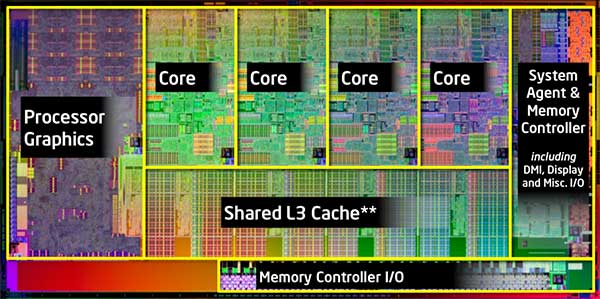
\includegraphics[width=2.5in]{die.png}
\caption{i7-2600 Die Layout}
\label{die}
\end{figure}
 
Each core of the i7-2600 has a 32KB data and instruction cache, a 256KB unified mid-level cache
and 2 level Data Translation Lookaside Buffer (DTLB) system of 64 and 512 entries. There is a single, 32 entry large page DTLB.
The cores in a socket share an inclusive last level cache that is 8MB and 16-way associative. ~\cite{levinthal2009}

The i7-2600 can perform four 64-bit floating point operations per cycle at peak performance.  At the 3.4GHz clock this equates to 13.6 billion floating point operations per second (GFLOPS) per core.  The processor has the ability, named Intel\textregistered Turbo Boost Technology 2.0, to increase its clock rate dynamically up to 3.8GHz if its operating below power, current, and temperature specification limits ~\cite{intel2012:turbo}.  This results in a peak performance of 15.2 GFLOPS per core.  The Turbo Boost ability is controlled in the system BIOS which is limited access in the Alamode Laboratory and could not be disabled in the test configuration.  The occurrence of the clock frequency increase is not predictable and is dependent on many uncontrollable factors.  Consequently, peak performance for experimental evaluation purposes will be reported as 13.6 GFLOPS but will actually range from 13.6 to 15.2 GFLOPS.

The test systems are 24 Dell Optiplex 990 desktop workstations in the Colorado School of Mines Alamode Computer Science Linux Laboratory in Brown Building room 136.
The systems are using an Ubuntu 10.04 operating system and all compilations are with the GNU gcc compiler version 4.4.3.  All experiments are run serially on a single core of the four core processor.  

\section{Baseline Matrix-Matrix Multiplication \\ (Question 2)}
Matrix-matrix multiplication ($C=C+A*B$) can be performed using the following simple triple loop:

Random 64-bit floating point square matrices of sizes 500, 1000, 1500, 2000, 2500, 3000, 3500, 4000, 4500, and 5000 were used in the experiments.

\section{Baseline Benchmark \\ (Question 3)}

\section{-O1 Optimization Benchmark \\ (Question 4)}

\section{-O2 Optimization Benchmark \\ (Question 5)}

\section{-O3 Optimization Benchmark \\ (Question 6)}

\section{-O3 -funroll-loops Optimization Benchmark \\ (Question 7)}

\section{Software Optimizations \\ Question 8}
\subsection{Step00}
\subsection{Step01}
\subsection{Step02}
\subsection{Step03}
\subsection{Step04}
\subsection{Step05}


\section{Conclusion}

...



% Reminder: the "draftcls", not "draft", class option should be used if
% it is desired that the figures are to be displayed while in draft mode.

% An example of a floating figure using the graphicx package.
% Note that \label must occur AFTER (or within) \caption.
% For figures, \caption should occur after the \includegraphics.
%
%\begin{figure}
%\centering
%\includegraphics[width=2.5in]{myfigure.eps}
%\caption{Simulation Results}
%\label{fig_sim}
%\end{figure}


% An example of a double column floating figure using two subfigures.
% (The subfigure.sty package must be loaded for this to work.)
% The subfigure \label commands are set within each subfigure command, the
% \label for the overall fgure must come after \caption.
% \hfil must be used as a separator to get equal spacing
%
%\begin{figure*}
%\centerline{\subfigure[Case I]{\includegraphics[width=2.5in]{subfigcase1.eps}
%\label{fig_first_case}}
%\hfil
%\subfigure[Case II]{\includegraphics[width=2.5in]{subfigcase2.eps}
%\label{fig_second_case}}}
%\caption{Simulation results}
%\label{fig_sim}
%\end{figure*}



% An example of a floating table. Note that, for IEEE style tables, the
% \caption command should come BEFORE the table. Table text will default to
% \footnotesize as IEEE normally uses this smaller font for tables.
% The \label must come after \caption as always.
%
%\begin{table}
%% increase table row spacing, adjust to taste
%\renewcommand{\arraystretch}{1.3}
%\caption{An Example of a Table}
%\label{table_example}
%\centering
%% The array package and the MDW tools package offers better commands
%% for making tables than plain LaTeX2e's tabular which is used here.
%\begin{tabular}{|c||c|}
%\hline
%One & Two\\
%\hline
%Three & Four\\
%\hline
%\end{tabular}
%\end{table}


% if have a single appendix:
%\appendix[Proof of the Zonklar Equations]
% or
%\appendix  % for no appendix heading
% do not use \section anymore after \appendix, only \section*
% is possibly needed

% use appendices with more than one appendix
% then use \section to start each appendix
% you must declare a \section before using any
% \subsection or using \label (\appendices by itself
% starts a section numbered zero.)
%
% Use this command to get the appendices' numbers in "A", "B" instead of the
% default capitalized Roman numerals ("I", "II", etc.).
% However, the capital letter form may result in awkward subsection numbers
% (such as "A-A"). Capitalized Roman numerals are the default.
%\useRomanappendicesfalse
%


% you can choose not to have a title for an appendix
% if you want by leaving the argument blank
%\section{}


% use section* for acknowledgement
%\section*{Acknowledgment}
% optional entry into table of contents (if used)
%\addcontentsline{toc}{section}{Acknowledgment}

%The authors would like to thank... This work was supported by the IEEE.

% trigger a \newpage just before the given reference
% number - used to balance the columns on the last page
% adjust value as needed - may need to be readjusted if
% the document is modified later
%\IEEEtriggeratref{8}
% The "triggered" command can be changed if desired:
%\IEEEtriggercmd{\enlargethispage{-5in}}

% references section
% NOTE: BibTeX documentation can be easily obtained at:
% http://www.ctan.org/tex-archive/biblio/bibtex/contrib/doc/

% can use a bibliography generated by BibTeX as a .bbl file
% standard IEEE bibliography style from:
% http://www.ctan.org/tex-archive/macros/latex/contrib/supported/IEEEtran/
%\bibliographystyle{IEEEtran.bst}
% argument is your BibTeX string definitions and bibliography database(s)
%\bibliography{IEEEabrv,../bib/paper}
%
\bibliography{csci564_term}
\bibliographystyle{IEEEtran}

% <OR> manually copy in the resultant .bbl file
% set second argument of \begin to the number of references
% (used to reserve space for the reference number labels box)

%\begin{thebibliography}{3}

%\bibitem{IEEEhowto:kopka}
%This is an example of a book reference
%H. Kopka and P.W. Daly, \emph{A Guide to {\LaTeX}}, third ed. Harlow, U.K.: Addison-Wesley, 1999.

%This is an example of a article reference
%A. Gefen, ``Simulations of Foot Stability During Gait Characteristic of Ankle Dorsiflexor Weakness
%in the Elderly,'' \emph{IEEE Trans. Neural Systems Rehabilitation Eng.,} vol. 9, no. 4, pp. 333-337, Dec. 2001.

%This is an example of a article from a conference proceeding
%T. Tuytelaars and L. van Gool ``Content-Based Image Retrieval Based on Local Affinely Invariant Regions,''
%\emph{Proc. Third Int'l Conf. Visual Information Systems,} pp. 493-500, 1999.

%Again, see the IEEEtrans_HOWTO.pdf for several more bibliographical examples. Also, more style examples
%can be seen at http://www.computer.org/author/style/transref.htm


%\end{thebibliography}



% biography section
%
% If you had an eps/pdf photo file (graphicx package needed)
% the extra braces prevent the LaTeX parser from getting confused
% when it sees the complicated \includegraphics command within an
% optional argument. You can create your own macro to make things
% simpler here.
%\begin{biography}[{\includegraphics[width=1in,height=1.25in,clip,keepaspectratio]{mshell.eps}}]{Michael Shell}
% or if you just want to reserve a space for a photo:

%\begin{biography}{Michael Shell}
%Biography text here.
%\end{biography}

% if you will not have a photo
%\begin{biographynophoto}{John Doe}
%Biography text here.
%\end{biographynophoto}

% insert where needed to balance the two columns on the last page
%\newpage

%\begin{biographynophoto}{Jane Doe}
%Biography text here.
%\end{biographynophoto}

% You can push biographies down or up by placing
% a \vfill before or after them. The appropriate
% use of \vfill depends on what kind of text is
% on the last page and whether or not the columns
% are being equalized.

%\vfill

% Can be used to pull up biographies so that the bottom of the last one
% is flush with the other column.
%\enlargethispage{-5in}

% that's all folks


\end{document}


